\documentclass[11pt]{article}
\usepackage[utf8]{inputenc}
\usepackage{amsmath,amssymb,amsthm} % for math stuff
\usepackage{enumitem} % itemsep
\usepackage{graphicx} % for pics
\usepackage[export]{adjustbox}
\usepackage[english]{babel}
\graphicspath{{./images/}}
\usepackage{caption}
\usepackage{mathtools}
\DeclarePairedDelimiter{\ceil}{\lceil}{\rceil}
\usepackage{indentfirst}
\usepackage{mathtools}
\setlength\parindent{0pt}
\usepackage{amsthm}
\theoremstyle{definition}
\newtheorem{definition}{Definition}[section]
\newtheorem{theorem}{Theorem}[section]
\newtheorem{corollary}{Corollary}[theorem]
\newtheorem{lemma}[theorem]{Lemma}
\theoremstyle{remark}
\newtheorem*{remark}{Remark}
\usepackage{tikz}
\usepackage{optidef}
\usepackage{hyperref}
\hypersetup{
    colorlinks=true,
    linkcolor=blue,
    filecolor=magenta,      
    urlcolor=blue,
}


\title{Guidance Laws in 3 body pursuit and evasion games}
\author{Dhruv Shah, Department of Electrical Engineering, IIT Bombay}
\date{ }

\begin{document}

\maketitle
\tableofcontents
\newpage
\section{Introduction}
The problem consists of three entities: an evading target denoted as
T, an attacking missile denoted as A, and a defending missile
denoted as D. We assume perfect information and analyze the
engagement in two dimensions.\\
\begin{figure}
    \centering
    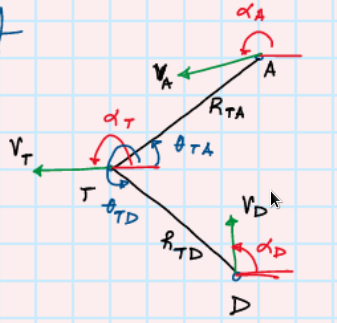
\includegraphics[width=0.6\textwidth]{tad_state_space.png}
    \caption{}
\end{figure}

\section{Problem Statement}\label{sec:2}
We have the following state space equations:  
\[
\begin{bmatrix}
\dot{R}_{TA} \\ R_{TA} \dot{\theta}_{TA}  \\ \dot{R}_{DT}  \\ R_{DT}\dot{\theta}_{DT}  \\ \dot{\alpha_A} \\  \dot{\alpha_D} \\ \dot{\alpha_T} 
\end{bmatrix}
=
\begin{bmatrix}
v_A cos(\alpha_A - \theta_{TA}) - v_T cos(\alpha_A - \theta_{TA}) \\
v_A sin(\alpha_A - \theta_{TA}) - v_T sin(\alpha_A - \theta_{TA}) \\
v_D cos(\alpha_D - \theta_{DT}) - v_T cos(\alpha_T - \theta_{DT}) \\
v_D sin(\alpha_D - \theta_{DT}) - v_T sin(\alpha_D - \theta_{DT}) \\
\frac{a_A}{v_A} u_A \\
\frac{a_D}{v_D} u_D \\
\frac{a_T}{v_T} u_T \\
\end{bmatrix}
\]

Thus, $|u_A| \leq 1$ , $|u_D| \leq 1$ and $|u_T| \leq 1$.  
The objective of the Defender team is to bring $R_{AD} < \varepsilon$ while maintaining $R_{TA} > \varepsilon$. Similarly the objective of the Attacker is to bring $R_{TA} < \varepsilon$ while maintaining $R_{AD} > \varepsilon$. Where $\varepsilon$ is the minimum safe distance.  


\section{Literature Survey}\label{sec:3}
Consider the control affine system of the form
\begin{equation} \label{eqn: control_affine}
 \dot{x} = f(x) + g(x) u \qquad x \in D, u \in U
\end{equation}
Define the Safe set by
\begin{equation} \label{eqn:safety}
    C_h := \{x \in D | h(x) \geq 0\}
\end{equation}
\begin{equation*}
    \partial C_h := \{x \in D | h(x) = 0\}
\end{equation*}
\begin{equation*}
    Int(C_h) := \{x \in D | h(x) > 0\}
\end{equation*}
In order to ensure the safety of the system i.e ensure $Int(C_h)$ is forward invariant we use the ZCBFs.

\begin{definition}[\cite{ames_2016_1}]
Consider \ref{eqn: control_affine} and $C_h$ , $h$ defined by \ref{eqn:safety}. A continuously differentiable function $h \colon Int(C_h) \to \mathcal{R} $ is called a Zeroing Control Barrier function (ZCBF) if there exists class $\kappa$ function $\alpha $ such that $\forall x \in Int(C_h)$
\begin{equation} \label{eqn: definition_RCBF}
    \sup_{u \in U} [L_fh(x) + L_gh(x)u + \alpha(h(x))]  \geq 0
\end{equation}
\end{definition}
Define $K_h(x)$ to be the set of admissible controls at x
\begin{equation}
    K_h(x) := \{u \in U | L_fh(x) + L_gh(x)u + \alpha(h(x))  \geq 0 \}
\end{equation}
\begin{figure}
    \centering
    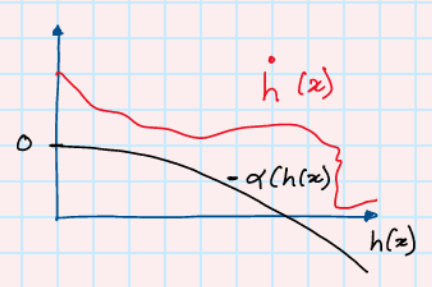
\includegraphics[width=0.4\textwidth]{tad_ZCBF.png}
\end{figure}
One can use QPs when one has a control objective and a safety objective that cannot be simultaneously satisfied to choose a control that mediates between the control objective and safety objective.\\
\begin{mini*}|s| % \usepackage{optidef}
{u}{||u(x) - \hat{u}(x)|| }{}{}
\addConstraint{L_fh(x) + L_gh(x)u(x) + \alpha(h(x))  \geq 0 }{}
\addConstraint{u(x) \in U}{}
\end{mini*}
where $\hat{u}(x) \in U$ is the nominal control that would ensure that the control objective is satisfied.\\
Define 
\begin{equation} \label{eqn:barrier_function_construction}
h(x(t);\rho , \gamma ) := \inf_{\tau \in [0,\infty]} \rho (\hat{x}(t + \tau))
\end{equation}
where $\rho$ is the safety function i.e $C := \{x \in D | \rho(x) > 0 \}$ and $\gamma$ is some nominal safety control i.e the system can use $\gamma$ to ensure its safety.
\begin{equation*}
    \hat{x}(t) = x(t) + \int_{0}^{\tau} \gamma(\hat{x}(s))ds
\end{equation*}
We can see that $h(x(t);\rho , \gamma )$ is a valid ZCBF.
\begin{align*}
    \dot{h} &= L_fh(x) + L_gh(x)\gamma(x)\\
            &= \lim_{a \xrightarrow{} 0^+} \frac{1}{a} [\inf_{\tau \in [a,\infty]} \rho (\hat{x}(t + \tau)) - \inf_{\tau \in [0,\infty]} \rho (\hat{x}(t + \tau))]\\
            & \geq 0
\end{align*}
Hence $\gamma(x) \in K_h(x) \quad \forall \quad x \in C_h$ which implies that h is a valid ZCBF.

\section{Approach 1: TAD as a Safety Critical QP}\label{sec:4}
Let $\hat{u}_A(x)$ be some guidance law that enables pure-pursuit of the target by the attacker.\\
Let $h(x)$ be an appropriately defined ZCBF.
\begin{mini*}|s| % \usepackage{optidef}
{u}{||u(x) - \hat{u}(x)|| }{}{}
\addConstraint{L_fh(x) + L_gh(x)u(x) + \alpha(h(x))  > 0 }{}
\addConstraint{|u(x)| \leq 1}{}
\end{mini*}
Note: This is a pointwise optimisation problem.\\
\begin{equation*}
h(x(t);\rho , \gamma ) := \inf_{\tau \in [0,\infty]} \rho (\hat{x}(t + \tau))
\end{equation*}
we need to chose $\rho$ and $\gamma$ appropriately.\\

One strategy is to chose $\gamma$ in a greedy way that drives the system towards the direction of maximum increase in $h(x)$ i.e in the direction of $\nabla h(x)$.\\
A way to do this would be to point the tangent vector of the system in the direction closest to that of $\nabla h(x)$.\\
However in our case, the tangent vector has the form
\begin{bmatrix}
0 \\ 
0 \\ 
0 \\ 
0 \\ 
u_A \\ 
0 \\ 
0 \\ 
\end{bmatrix}\\
Clearly this wont give good results as the control does not directly affect the states but does it through some integrator layers.\\
We need a different approach to choose $\gamma$.\\

We use two choices of $\rho$ in our simulations.\\
1] $\rho(x) = ((x_A - x_D)^2 + (y_A - y_D)^2)^{1/2}$\\
\begin{figure}
    \centering
    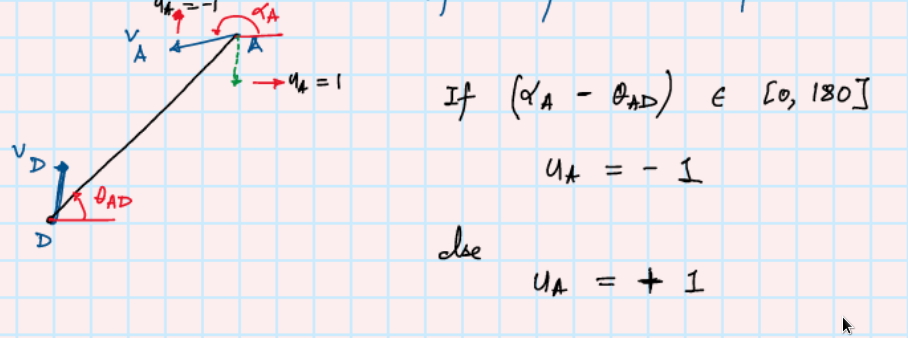
\includegraphics[width=1\textwidth]{tad_approach1_1.png}
    \caption{Choice of $\gamma$}
\end{figure}
2] $\rho(x) = \Delta \theta(x) = |\theta_{TA} - \theta_{DT}|$\\
As shown in \cite{shima} if the defender is able to position itself on the LOS joining A and T, then the defender has won. Thus, this safety function tries to ensure that $\Delta \theta(x)$ which is the angle between TA and TD does not fall below a threshold.
\begin{figure}
    \centering
    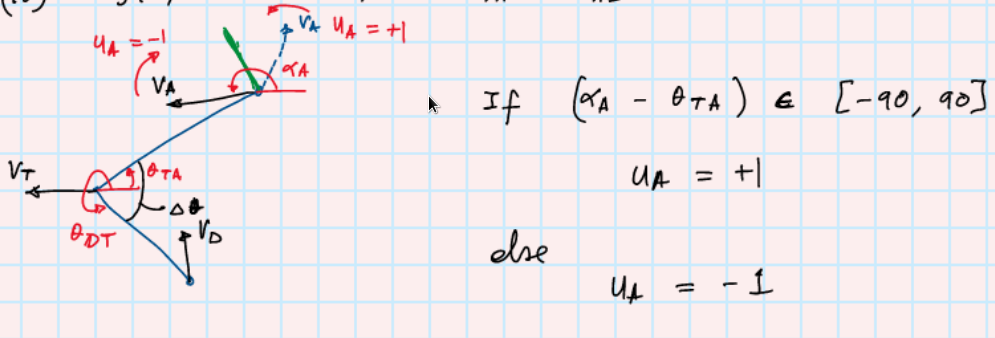
\includegraphics[width=1\textwidth]{tad_approach1_2.png}
    \caption{Choice of $\gamma$}
\end{figure}


\section{Simulations}\label{sec:5}
\begin{figure}
    \centering
    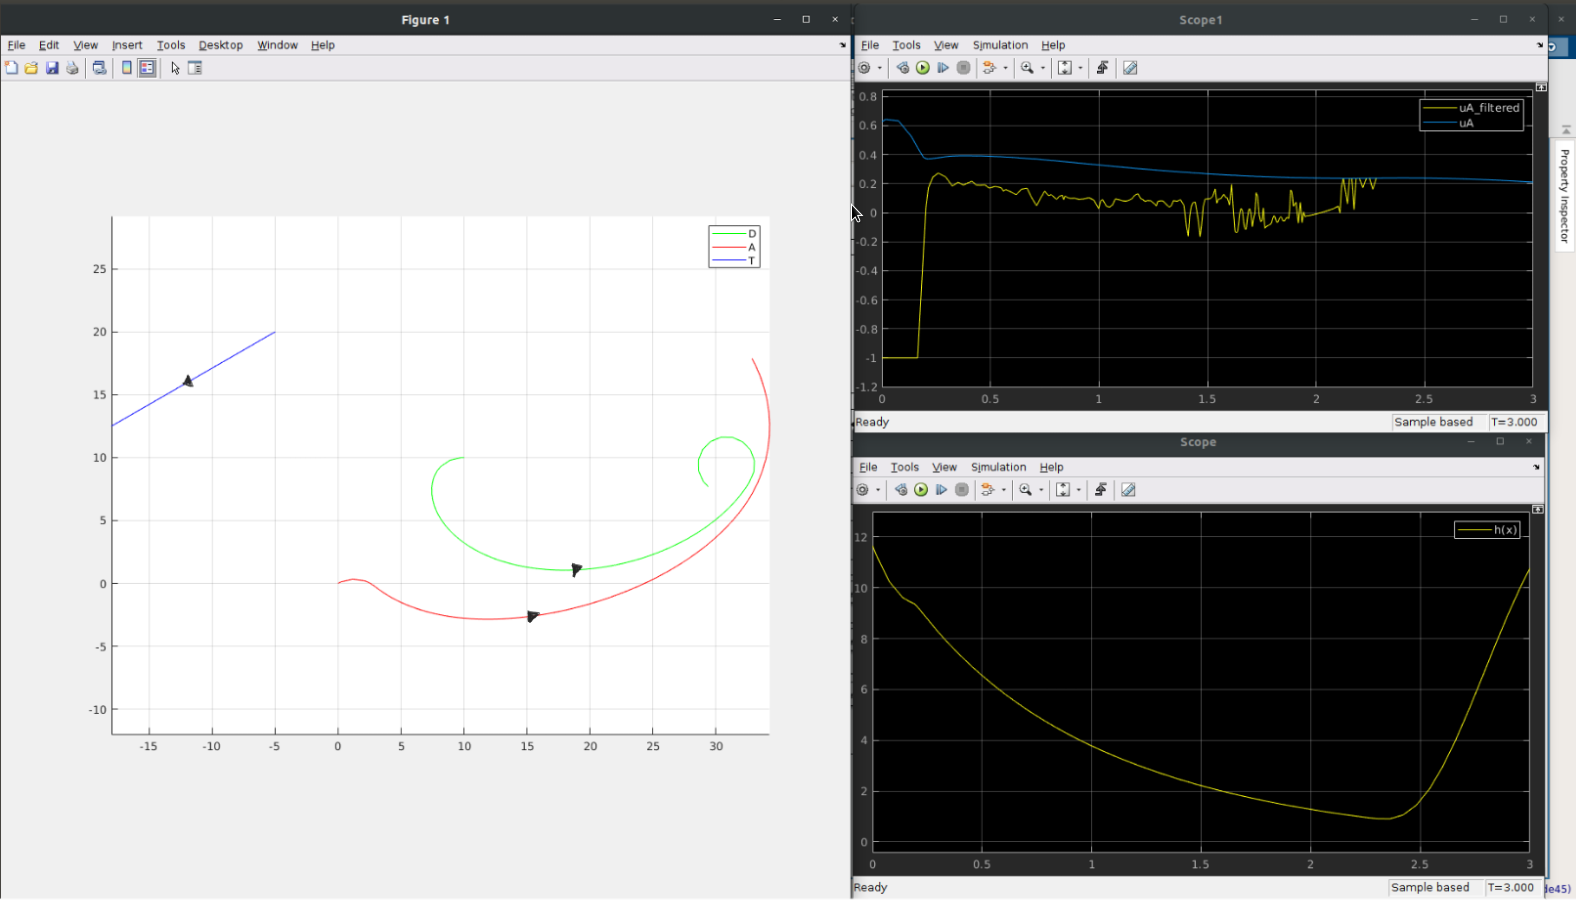
\includegraphics[width=1\textwidth]{sim2_case1.png}
    \caption{Attacker is successfully able to evade the Defender while pursuing the Target using 1st safety function}
\end{figure}

\begin{figure}
    \centering
    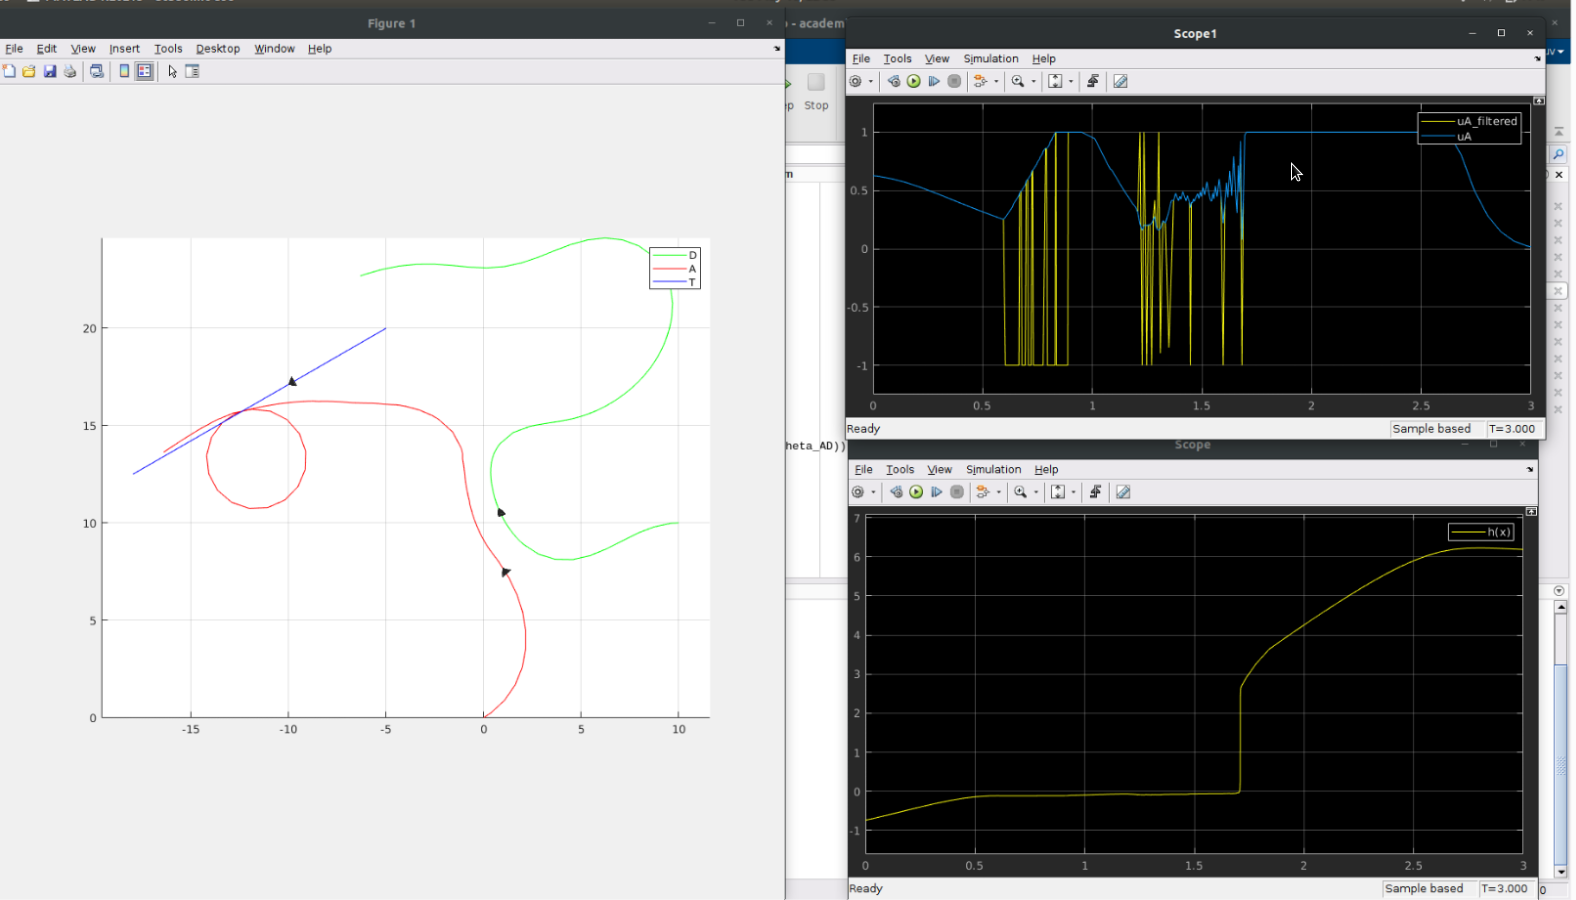
\includegraphics[width=1\textwidth]{sim2case2.png}
    \caption{Attacker is successfully able to evade the Defender while pursuing the Target using 2nd safety function}
\end{figure}

\section{Approach 2 : Using Time of Engagement}\label{sec:6}
Let $T(x)$ be the time required for the attacker to capture the target with the initial state being $x$.
\begin{equation} \label{eqn:time_to_go_h}
    h(x(t);\rho , \gamma) := \inf_{\tau \in [0,T(x)]} \rho (\hat{x}(t + \tau))
\end{equation}
where $\gamma$ is some guidance law where the attacker pursues the target ignoring the defender and $h$ is the minimum separation between the attacker and defender under $\gamma$ over the finite time horizon.\\
\begin{figure}
    \centering
    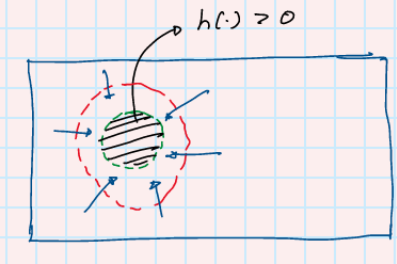
\includegraphics[width=0.4\textwidth]{tad_approach2.png}
\end{figure}

Case 1] $h(x(t);\rho , \gamma) > \varepsilon$\\
Capture is ensured and we are done\\

Case 2] $h(x(t);\rho , \gamma) \leq \varepsilon$\\
\begin{enumerate}
    \item In this case we need to design a maneuver say $E(x)$ for the attacker to move in a way that increases the value of h(x) until $h(x) > \varepsilon$.\\
    \item One way to do this would be to steer the system using the tangent vector in the direction of $\nabla h(x)$. However as described above, the system under consideration is not steerable using the tangent vector.\\
    \item As done in the previous case (using the physical understanding of h(x)), one could use a guidance law where the attacker purely evades the defender. However there is no guarantee that this is the optimal choice. Thus, this remains a further area of research.
\end{enumerate}

\section{Future Work} \label{sec:7}
\subsection{Future Work : Numerical Studies}
\begin{enumerate}
    \item Under Approach 1, simulations need to be conducted with different choices of nominal guidance strategies and varying initial conditions.\\
    \item Furthermore, these simulations need to be compared with the existing literature for the TAD problem (Specifically those implementing cooperative guidance against the attacker).
    \item Under Approach 2, various heuristic based maneuvers E(x) need to be evaluated using simulations and their performance compared with that of Approach 1.\\
\end{enumerate}
\subsection{Future Work: Theoretical Investigations}
\begin{enumerate}
    \item An open challenge to obtain a closed-form expression of the barrier function for the system under consideration still prevails. One could also characterize the capture regions numerically if a closed-form expression for a ZCBF is available.\\
    \item Designing the maneuver $E(x)$ with a theoretically sound justification remains to be explored. One could use ideas from backstepping to steer the system in the direction of $\nabla h(x)$ or explore something completely different.
\end{enumerate}
  
\section{Conclusion}\label{sec:8}
The economic dispatch problem has been studied in this paper for a class of smart grids subject to unknown communication uncertainties by employing adaptive consensus-based dispatch algorithms. Distributed consensus-based power dispatch algorithms are developed to achieve optimal dispatch of active power by appropriately sharing the load among generating units while guaranteeing consensus among individual incremental costs. A new kind of distributed adaptive weight-adjustment approach is designed and utilized to select the communication weights among neighboring generating units such that consensus of incremental costs for generating units under both cases.\\
\section{References}\label{sec:9}
\begin{thebibliography}{00}
\bibitem{ames_2016_1}A. D. Ames, X. Xu, J. W. Grizzle, and P. Tabuada, “Control barrier function based quadratic programs with application to automotive safety systems,” 2016.
\bibitem{2}E. Squires, P. Pierpaoli and M. Egerstedt, "Constructive Barrier Certificates with Applications to Fixed-Wing Aircraft Collision Avoidance," 2018 IEEE Conference on Control Technology and Applications (CCTA)
\bibitem{16} D. G. Luenberger, Optimization by vector space methods. John Wiley & Sons, 1969
\bibitem{shima}Ratnoo and Shima, "Line-of-Sight Interceptor Guidance for Defending an Aircraft",2011 Journal of Guidance, Control, and Dynamics
\bibitem{last}\href{https://github.com/dhruvshah0208/TAD}{Github Repository}

\end{thebibliography}

\vspace{12pt}
\color{red}



\end{document}